\documentclass[
	emulatestandardclasses, % prevent scrartcl from fucking up
	11pt,
	% titlepage,
	a4paper,
	toc=bib, % add bibliography to table of contents
	parskip=half-,
	numbers=endperiod,
]{scrartcl}

\usepackage{./basix}

\title{Assignment 1.1}
\subtitle{Intelligent Virtual Environments}
\author{Antonio José Fernández Pinto \and Luis Fernando Choque Arana}
\date{} % do not put the date in the title

\begin{document}

\maketitle[0]

\vspace{-1cm}

\section{Play Instructions}

This is a shooter game where you have to shoot only enemies and not allies within a time limit. Enemies are represented as squares and allies are represented as capsules. The former gives 1 point when shooting it and the latter -1 point. From the start of the game, enemies and allies will randomly appear and disappear until the time limit (60 seconds) ends. Your score and remaining time are shown in the upper left corner of the screen.

The controls are simple. You can use either WASD or arrow keys to move around, both left and right shift make you run, moving the mouse rotates the camera and left clicking shoots a bullet.

The logs are stored in a \texttt{log.txt} file in whatever directory you run the executable.

\section{Project Structure}

Apart from the \texttt{Materials} and \texttt{Prefabs} folders in \texttt{Assets}, which contain expected and not that interesting files, these are the important folders.

\subsection{Scenes}

The game only contains one scene, that is structured as follows:

\begin{itemize}
	\item \textbf{Directional Light}. Our little sun.
	\item \textbf{Player}. The game object representing the player.
	\begin{itemize}
		\item \textbf{Main Camera}. The camera game object. It holds the \texttt{CameraController} script.
		\begin{itemize}
			\item \textbf{Gun}. The game object that spawns the bullets. It holds the \texttt{GunController} script.
		\end{itemize}
	\end{itemize}
	\item \textbf{Canvas}. The general UI game object.
	\begin{itemize}
		\item \textbf{Panel}. A black rectangle below the UI text.
		\item \textbf{Score}. A text showing the current score.
		\item \textbf{Clock}. A text showing the remaining time. It also holds the \texttt{Timer} script.
		\item \textbf{Watchout}. The text shown at the beginning of the game.
	\end{itemize}
	\item \textbf{Event System}. It holds the \texttt{Logger} script.
	\item \textbf{NPC Spawner}. The game object that spawns enemies and allies. It holds the \texttt{NPCController} script.
	\item \textbf{Grass}. A grass object to serve as floor and reference point.
\end{itemize}

\subsection{Scripts}

\begin{itemize}
	\item \textbf{BulletController}. A simple script for each bullet that detects collisions with allies/enemies, destroys them and updates the score.
	\item \textbf{CameraController}. General player movement.
	\item \textbf{GunController}. Spawns bullets when needed.
	\item \textbf{Logger}. General logging to a text file.
	\item \textbf{NPCController}. Spawns and despawns enemies and allies.
	\item \textbf{Timer}. Keeps track of remaining time and updates the UI accordingly.
\end{itemize}

\subsection{Other folders}

\begin{itemize}
	\item \textbf{Fonts}. Contains the Liberation Sans font that is used for the text. This was added to ensure compatibility with development environment on Linux.
	\item \textbf{LowPoly}. Contains the grass model used for the floor.
	\item \textbf{Textures}. Contains the grass texture used for the floor.
\end{itemize}

\section{Game Screenshots}

\begin{figure}[H]
	\centering
	\label{fig:start}
	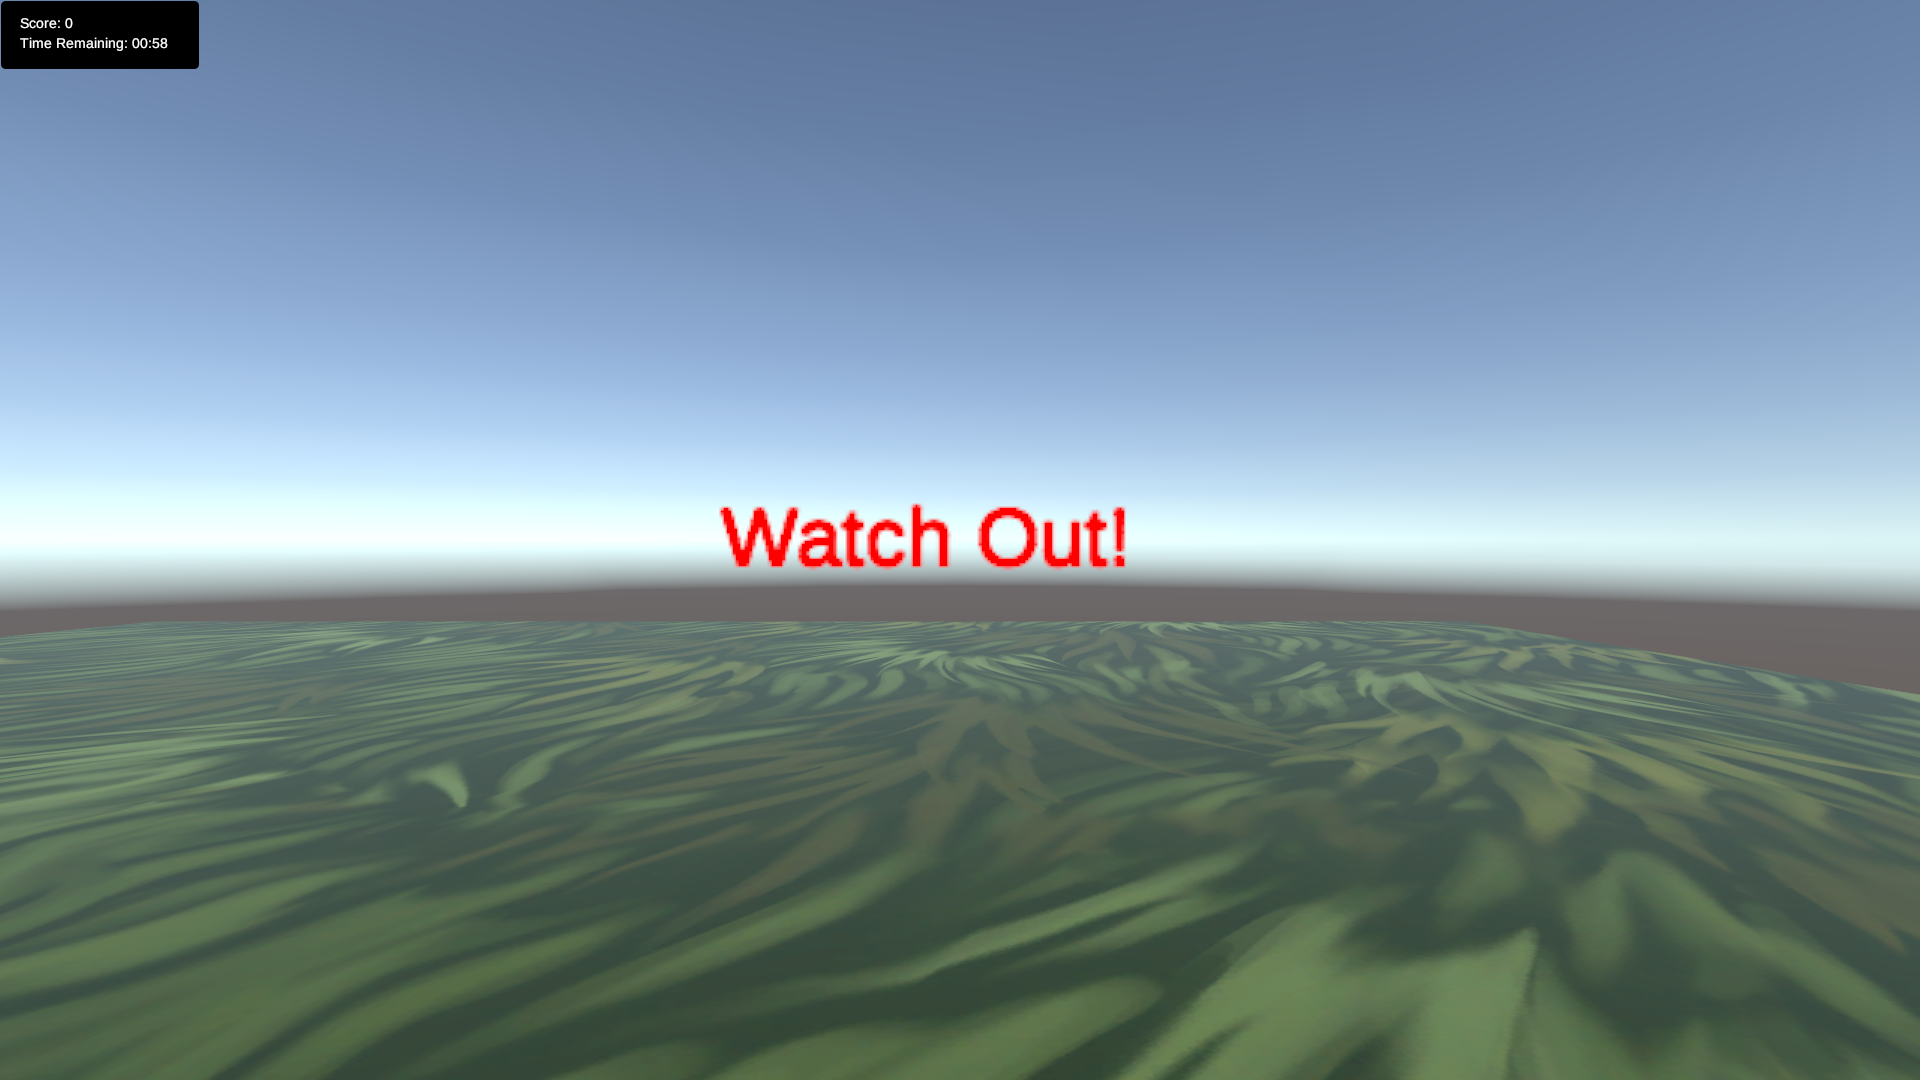
\includegraphics[width=0.75\linewidth]{start}
	\caption{Start of the game}
\end{figure}

\begin{figure}[H]
	\centering
	\label{fig:midgame}
	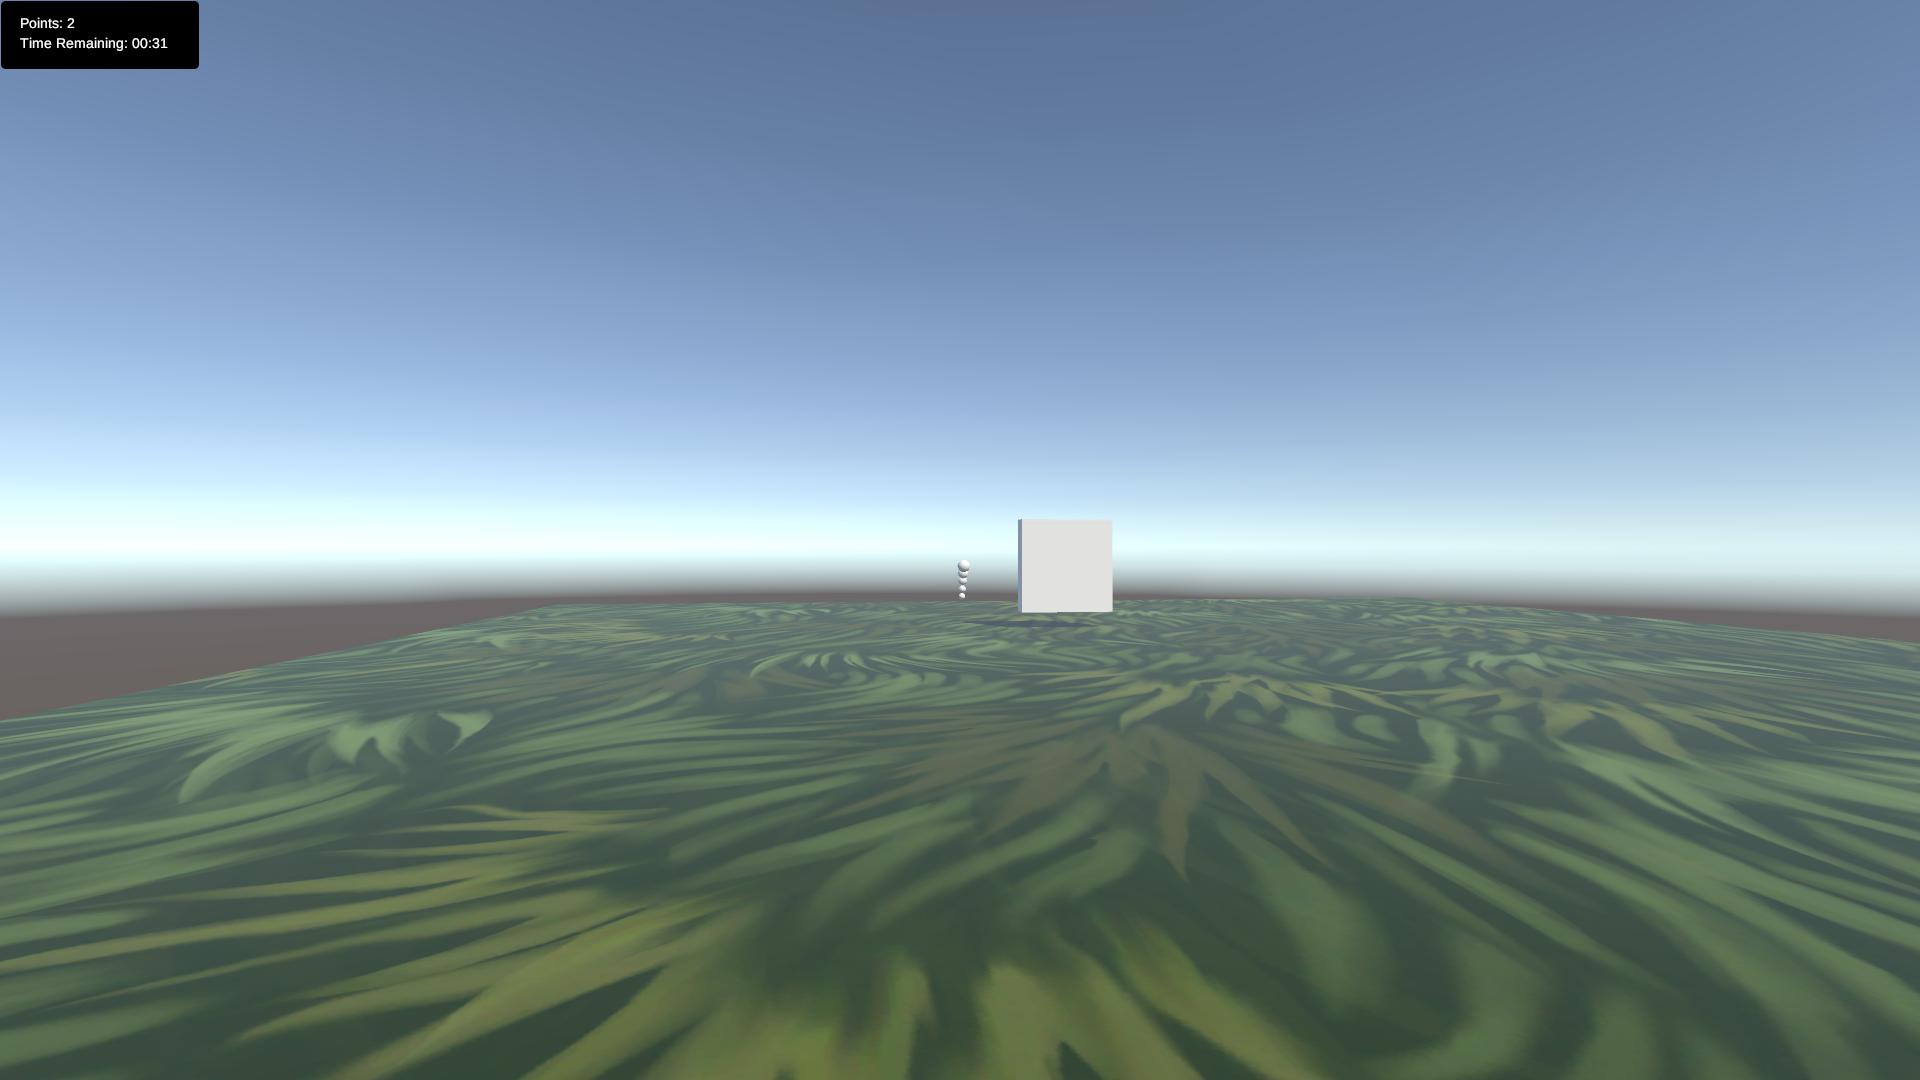
\includegraphics[width=0.75\linewidth]{midgame}
	\caption{Midgame}
\end{figure}

\end{document}
